\documentclass[titlepage]{article}
\usepackage[utf8]{inputenc}
\usepackage{graphicx}
\usepackage{amsmath}
\usepackage[english]{babel}
\usepackage[nottoc]{tocbibind}
\usepackage{hyperref}
\usepackage{float}

\title{Fashionable Neural Networks}
\author{Julius C Aguma (38208345), Matt Dees (30281707), James}
\date{December 2019}

\begin{document}

\maketitle

\section{Introduction}

\par For our final project we decided to explore the relationship between capacity and accuracy for two types of neural networks: the feedforward neural network and the convolutional neural network. The two neural networks were trained on the Fashion-MNIST dataset \cite{fashionmnist}, and thus, the input to our neural networks is one $28 \times 28$ image and the output is a classification (1-10) for that image. We measured the ratio of correct test image classifications to total number of test images as a way of measuring the strength of the neural network as capacity was varied. 

\section{Dataset}

\begin{figure}[h!]
\centering
  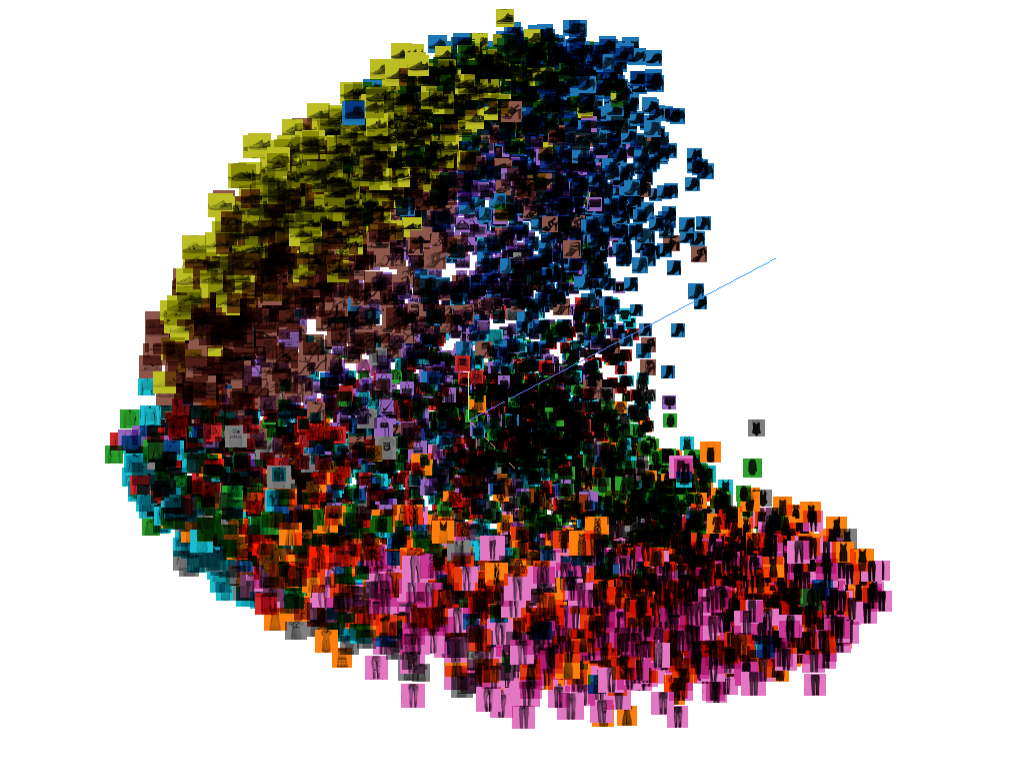
\includegraphics[scale=.25]{tensorboard_pca.png}
  \caption{Tensorboard visualization of the Fashion-MNIST dataset.}
  \label{fig:tensorboard_pca}
\end{figure}

\par We decided to use the Fashion-MNIST dataset created by Zalando Research due to the excellent documentation on Github and plethora of utilities available within their Github repository. The dataset consists of a training set and validation set. The training set contains 60,000 images while the validation set contains 10,000 images. Each image is a $28 \times 28$ grayscale image (784 total pixels). The training set is of the form $X = Y$, where $X$ is a $60,000 \times 784$ matrix and $Y$ is a $60,000 \times 1$ matrix. Each row in $X$ corresponds to a different image and each column corresponds to a pixel of that image (used as features). The $Y$ matrix is $60,000 \times 1$ matrix where each value is a classification for the corresponding row (image) in the $X$ matrix. Each classification is an integer value which maps to one of 10 different clothing classes.

\par To better understand our dataset, we decided to visualize it using Tensorboard \cite{tensorboard} and Matplotlib \cite{matplotlib}. Our implementation for visualizing the data is located in the \textbf{visualization.py} file in the top-level directory. We opted for a Principal Component Analysis to get a better idea of what clusters may exist amongst the data. We chose PCA because the data has a relatively high number of features (784), which is not easy to visualize. With PCA, we have access to the features the preserve the most variance in the data, and may offer some insight into how it can be organized. When loaded into the Tensorboard visualization suite we were able to observe images like in Figure \ref{fig:tensorboard_pca}. Once colored, it was evident that the data actually formed reasonable clusters. This led us to believe that data was reasonably separable, so we \textit{should} see fairly high classification rates with a model using the correct features. Using Matplotlib, we were also able to visualize a singular image. Upon visualizing a single image, it was obvious that we should normalize the data. Since each pixel is a value between 0 and 255, we decided to normalize the data by dividing each pixel by 255. The proved extremely helpful in getting better results from our neural networks.



\begin{figure}[h!]
\centering
  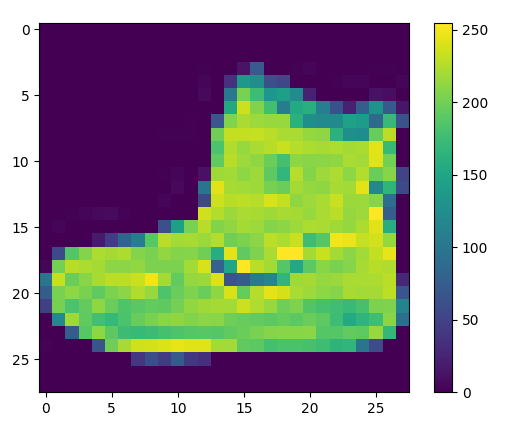
\includegraphics[scale=.33]{single_image.png}
  \caption{Image 0 from the Fashion-MNIST dataset visualized using a color map.}
  \label{fig:single_image}
\end{figure}


\section{Neural Network Models}
\par To analyse the capacity of neural network models on the fashion-mnist data, we chose to use a feedforward and convolutional neural network. While holding all other parameters constant, the number of hidden layers, $k$ was varied for values ${1,2,4,8}$. Results of this analysis are presented below with a summary of the architectures of both models.

\subsection{FeedForward }
\subsubsection{Architecture}
\par Using tensorflow with keras, we built a feedforward network that takes fashion mnist data as input read through the mnist-reader.py script. The network has $k$ hidden layers where $k$ is varied for an analysis of capacity, that is a comparison of deep vs shallow networks on the fashion-mnist dataset. The data is split into training and validation data as shown in the model parameters below and the model is trained for 50 epochs where each epoch has 40000 iterations. In addition we use dropout factors less than 1 for regularization and cross entropy as loss function with the adadelta optimizer as a learning rate method for our gradient descent. The hidden layers use relu for an activation function while the output layer uses softmax. All inputs are normalized. Below are parameters and results for each $k$ in the set ${1,2,4,8}$
\begin{figure}[H]
	\centering
	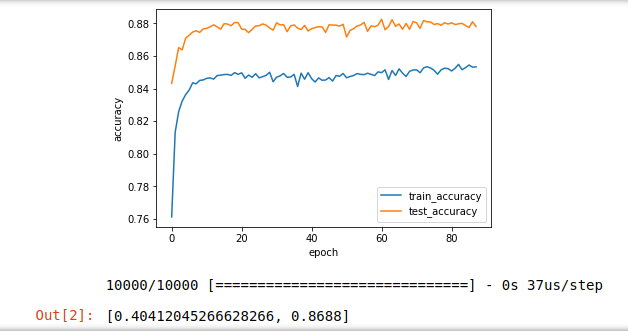
\includegraphics[width=1.0\textwidth]{1b.png}
	\caption{Feedforward neural network with $K = 1$.}
\end{figure}
\begin{figure}[H]
	\centering
	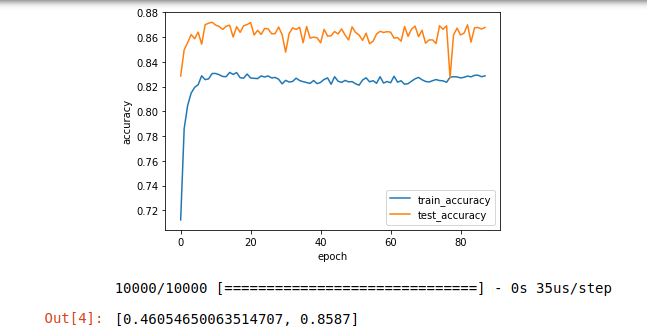
\includegraphics[width=1.0\textwidth]{2b.png}
	\caption{Feedforward neural network with $K = 2$.}
\end{figure}
\begin{figure}[H]
	\centering
	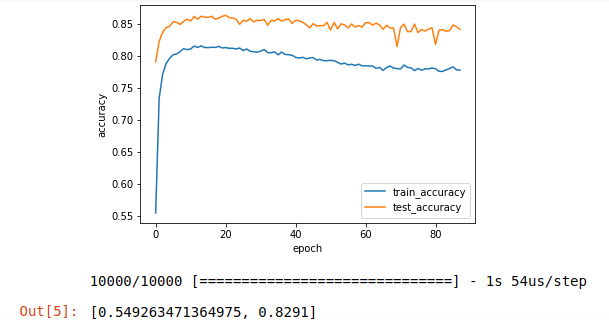
\includegraphics[width=1.0\textwidth]{4b.png}
	\caption{Feedforward neural network with $K = 4$.}
\end{figure}
\begin{figure}[H]
	\centering
	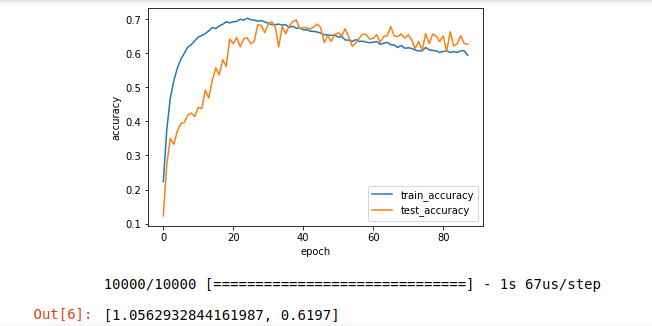
\includegraphics[width=1.0\textwidth]{8b.png}
	\caption{Feedforward neural network with $K = 8$.}
\end{figure}

\subsection{Convolutional model}
\subsubsection{Architecture}
\par The convolutional model(cnn) is similar to the feedforward model in number of hidden layers, optimizer, regularization, activation functions, and validation. However, the  cnn also has 2 3x3 convolutional  filters and a 2x2 max pooling layer for downsampling the convolution layers. Results follow below.

\begin{figure}[H]
	\centering
	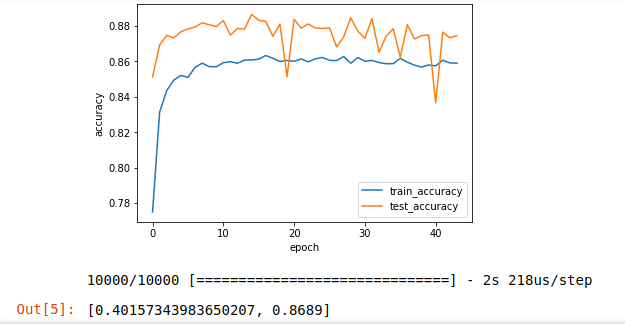
\includegraphics[width=1.0\textwidth]{cb.png}
	\caption{Convolutional neural network with $K = 1$.}
\end{figure}
\begin{figure}[H]
	\centering
	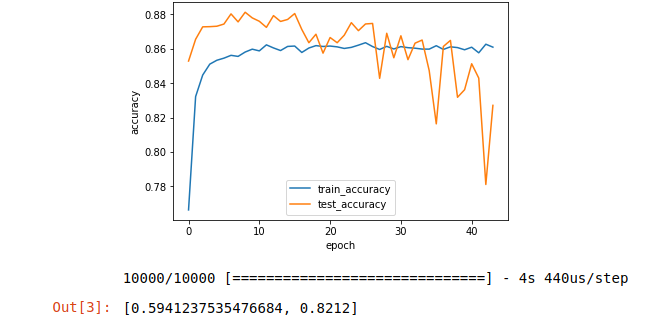
\includegraphics[width=1.0\textwidth]{c1b.png}
	\caption{Convolutional neural network with $K = 2$.}
\end{figure}
\begin{figure}[H]
	\centering
	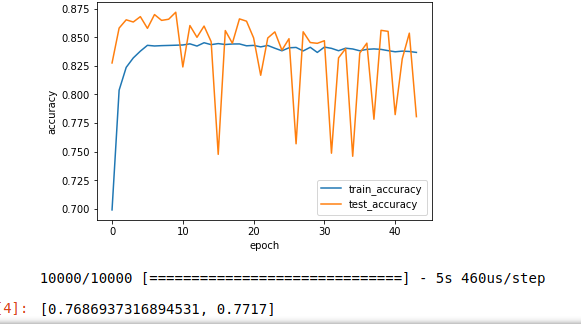
\includegraphics[width=1.0\textwidth]{c4b.png}
	\caption{Convolutional neural network with $K = 4$.}
\end{figure}


\subsection{Discussion of results}
\par The feedforward model gave more consistent predictions with a smoother curve while the cnn gave us higher accuracy with a peak of about 90\%. For both architectures, the rate of overfitting increased with increase in the number of hidden layers. More so for the cnn where by k = 4 we see an overwhelming amount of overfitting. We also see that the peak accuracy never increased with increase in number of hidden layers. Further proving the known fact that capacity of a neural network doesnot increase with deeper networks but only the type of functions that can be estimated improves. A good next step in the capacity study would be to look at how the network performance changes with wider hidden layer, that is hidden layers with more neurons.


\bibliographystyle{unsrt}
\bibliography{references}

\end{document}
